% !TEX TS-program = pdflatex
% !TEX encoding = UTF-8 Unicode

\documentclass[10pt]{article}

%%% PACKAGES
\usepackage[utf8]{inputenc}
\usepackage{booktabs}
\usepackage{array}
\usepackage{paralist}
\usepackage{verbatim}
\usepackage[T1]{fontenc}
\usepackage[english]{babel}
\usepackage{sectsty}
\usepackage{graphicx}
\usepackage{geometry}
\usepackage{fancyhdr}
\usepackage[nottoc,notlof,notlot]{tocbibind}
\usepackage{amsmath}
\usepackage[table,xcdraw]{xcolor}
\usepackage{subcaption}
\usepackage{caption}
\usepackage{lmodern}
\usepackage[colorlinks=true, linkcolor=blue]{hyperref}
\usepackage{float}
\usepackage{booktabs}
\usepackage{multirow}
\usepackage{amssymb}
\usepackage{microtype}
\usepackage{seqsplit}
\usepackage{longtable}
%%% Margini Personalizzati
\geometry{
  a4paper,
  top=2.5cm,
  bottom=2.5cm,
  left=2.5cm,
  right=2.5cm
}

%%% Header & Footer
\pagestyle{fancy}
\fancyhf{}
\fancyfoot[C]{\thepage}

%%% Stile sezioni
\allsectionsfont{\sffamily\bfseries}

%%% Table of Contents

\begin{document}
\setlength{\parindent}{0pt}    % Nessuna indentazione a inizio paragrafo
\setlength{\parskip}{6pt}

%%% Copertina
\begin{titlepage}
    \centering
    \vspace*{2cm}
    
    
\includegraphics[width=0.4\textwidth]{image.jpg}\par
    \vspace{1.5cm}
    
    {\scshape\Large Corso di Data Mining 1 \par}
    
    \vspace{2cm}
    {\huge\bfseries DataMining1\_Report \par}
    
    \vspace{2.5cm}
    {\Large\itshape Clarissa Rizzello\par}
    \vspace{0.5cm}
    {\Large\itshape Lavinia Rotellini\par}
    \vspace{0.5cm}
    {\Large\itshape Rachele Sabbatini\par}
    
    \vfill
\end{titlepage}

\tableofcontents
\newpage

\section{Introduction}
In this study, we conducted a data mining analysis on an IMDb dataset. We began with a data understanding phase, exploring and preparing the dataset’s attributes to gain deeper insights. Subsequently, we applied various clustering algorithms, including K-Means, DBSCAN, and Hierarchical Clustering. Following clustering, we progressed to classification, training multiple models such as K-Nearest Neighbors (KNN), Naïve Bayes, and Decision Trees. Our exploration also extended to regression analysis, and finally, we employed association rule mining techniques, specifically Apriori and FP-Growth algorithms, to identify meaningful patterns within the data.
\section{Data Understanding}
This dataset from IMDb contains information about movies and TV shows, including key attributes such as titles, release years, runtimes, user ratings, awards, and genres.
\subsection{Data Semantics}
Our datase was composed of 16430 records with 23 descriptive features. The features were both categorical (\textit{qualitative}) and numeric (\textit{quantitative}). Table \ref{tab:feature_description} summarizes the key features of the dataset.
\setlength{\tabcolsep}{6pt} % spazio orizzontale tra colonne
\renewcommand{\arraystretch}{1.3} % altezza riga aumentata per leggibilità

\begin{center} % per centrare la tabella, opzionale
\begin{longtable}{| >{\ttfamily}p{5cm} | p{4cm} | p{7cm} |}
\caption{Feature descriptions and types} \label{tab:feature_description} \\
\hline
\textbf{Feature} & \textbf{Feature Type} & \textbf{Description} \\
\hline
\endfirsthead

\hline
\textbf{Feature} & \textbf{Feature Type} & \textbf{Description} \\
\hline
\endhead

\hline
\multicolumn{3}{r}{\textit{Continued on next page}} \\
\endfoot

\hline
\endlastfoot

originalTitle & Categorical, Nominal & Original title of the work, expressed in the original language. \\
\hline
runtimeMinutes & Numeric (integer) & Primary runtime of the title, expressed in minutes. \\
\hline
isAdult & Categorical, Binary & Binary indicator specifying whether the content is adult (1) or not (0). \\
\hline
startYear & Numeric, Discrete & Release year of the title; for TV series, the start year of the series. \\
\hline
endYear & Numeric, Discrete & TV Series end year, if applicable. \\
\hline
numVotes & Numeric, Discrete & Total number of votes received by the title. \\
\hline
numRegions & Numeric, Discrete & Number of geographic regions where this version of the title is available. \\
\hline
worstRating & Numeric, Interval & Lowest possible rating value assigned to the title, minimum on the rating scale. \\
\hline
bestRating & Numeric, Interval & Highest possible rating value assigned to the title, maximum on the rating scale. \\
\hline
canHaveEpisodes & Categorical, Binary & Indicates whether the title can include episodes. \\
\hline
isRatable & Categorical, Binary & Indicates whether the title can be rated by users. \\
\hline
totalImages & Numeric, Discrete & Total number of images associated with the title’s IMDb page. \\
\hline
totalVideos & Numeric, Discrete & Total number of videos associated with the title’s IMDb page. \\
\hline
totalCredits & Numeric, Discrete & Total number of credits associated with the title. \\
\hline
criticReviewsTotal & Numeric, Discrete & Total number of professional critic reviews. \\
\hline
awardWins & Numeric, Discrete & Total number of awards won by the title. \\
\hline
awardNominationsExcludeWins & Numeric, Discrete & Total number of award nominations excluding wins. \\
\hline
titleType & Categorical, Nominal & Category or format of the title (e.g., movie, short, TV series, episode, video). \\
\hline
rating & Numeric, Ratio & Average IMDb rating of the title. \\
\hline
ratingCount & Numeric, Discrete & Total number of user ratings submitted for the title. \\
\hline
countryOfOrigin & Categorical, Multi-valued Nominal & Country where the title was primarily produced. \\
\hline
genres & Categorical, Multi-valued Nominal & Genres associated with the title. \\
\hline
userReviewsTotal & Numeric, Discrete & Total number of user-written reviews. \\
\hline
\end{longtable}
\end{center}
 Table \ref{tab:feature_description} summarizes the key features of the dataset.
\subsection{Data Quality and Correlations}
\subsection{Distribution and Statistics}
\subsection{Outliers}
\subsection{Particular Values}
\subsection{Data Transformation}

\section{Clustering}
In this section we provide the results of the clustering analysis, which was performed using the following algorithms:

\begin{itemize}
    \item\textbf{KMeans}, from the family of instance-base clustering algorithms
    \item\textbf{DBScan}, from the family of density-based clustering algorithms
    \item\textbf{HDBScan}, from the family of density-based clustering algorithms
    \item\textbf{Agglomerative (or hierarchical) Clustering}. This last method was applied both with and without the connectivity constraint, and in all of the different versions: Single Link, Average Link, Complete Link and Ward.
    \item\textbf{Kmodes}, to cluster on categorical features.
\end{itemize}

\subsection{Preprocessing towards clustering}
The dataset used for clustering analysis was derived from the one prepared during the data understanding phase, with additional preprocessing tailored to the requirements of each clustering algorithm.
A key consideration in preprocessing was the type of features required by the algorithms. Algorithms such as KMeans, DBSCAN, HDBSCAN, and Agglomerative Clustering operate on numerical features, while KModes is specifically designed for categorical data. Accordingly, the dataset was preprocessed in two different ways to accommodate these distinctions.
For the algorithms requiring numerical input, all features of type 'object' and 'boolean' were removed. These included: \texttt{originalTitle}, \texttt{titleType}, \texttt{canHaveEpisodes}, \texttt{countryOfOrigin}, and \texttt{genres}. Additionally, the decade column—though numerical—was excluded because it represents a categorical concept and is not meaningful in a distance-based analysis. The columns \texttt{userReviewsTotal} and \texttt{criticReviewsTotal} were also dropped, as their information was already incorporated into the \texttt{totalReviews} feature.
The dataset was therefore now composed of the following features: 

The main focus of this analysis was to understand how different types of preprocessing affected the performance of various clustering algorithms, and to identify which preprocessing methods were most appropriate for our dataset. To this end, feature transformations were applied in four different ways:
\begin{itemize}
	\item The first transformation applied MinMax scaling only
	\item The second transformation combined both the MinMax scaling with a logarithmic transformation
	\item The third transformation used Standard scaling alone
	\item The fourth transformation combined Standard scaling with a logarithmic transformation	
\end{itemize}

As for KModes, the dataset was preprocessed by deleting all the numerical features and keeping the following:\texttt{titleType}, \texttt{canHaveEpisodes}, \texttt{countryofOrigin}, \texttt{genres}, \texttt{decade}.

\subsection{Centroid-based Clustering: KMeans}

\begin{table}[ht!]
    \centering
    \begin{tabular}{|c|c|}
    \hline
    Preprocessing & K \\
    \hline
    MinMax & 4 \\
    MinMax+Log & 4 \\
    Standard Scaling & 5 \\
    Standard+Log & 3 \\
    \hline
    \end{tabular}
    \caption{KMeans Results - Elbow Method}
    \label{table:KM_K}
\end{table}
To determine the most appropriate number of clusters for our dataset, we applied the \textbf{Elbow Method}. he results indicated that different preprocessing techniques led to different optimal numbers of clusters, as summarized in Table \ref{table:KM_K}:
\begin{table}[ht!]
    \centering
    \begin{tabular}{|c|c|c|}
    \hline
    \multicolumn{3}{|c|}{KMeans Clustering Results} \\
    \hline
     & SSE & Silhouette Score \\
    \hline
    MinMax & 629.92 & 0.30 \\
    MinMax \& Log & 1723.69 & 0.17 \\
    Standard Scaling & 74678.86 & 0.24 \\
    Standard \& Log & 85385.59 & 0.24 \\
    \hline
    \end{tabular}
    \caption{KMeans Clustering Results}
    \label{table:KM}
\end{table}
However, the clustering results across these methods were generally suboptimal and varied significantly. Table \ref{table:KM} shows the Sum of Squared Errors (SSE) and silhouette scores for each preprocessing approach:
These results clearly indicate that our dataset is not well-suited for clustering, as evidenced by the relatively high SSE values and silhouette scores far from the ideal benchmark of 1. Low silhouette scores suggest poor cluster cohesion and separation, implying that the inherent structure of the data does not strongly support meaningful clusters.
\subsection{Density-based Clustering}

\subsubsection{DBScan}

To determine an appropriate value for the epsilon ($\epsilon$) parameter in the DBSCAN algorithm, we initialized a range of candidate $\epsilon$ values and evaluated how many clusters each generated, along with their corresponding silhouette scores.
\begin{table}[ht!]
    \centering
    \begin{tabular}{|c|c|c|}
    \hline
    \multicolumn{3}{|c|}{DBScan Clustering Results} \\
    \hline
     Preprocessing & $\epsilon$ & Silhouette Score \\
    \hline
    MinMax & 0.3 & 0.57 \\
    MinMax \& Log & 0.3 & 0.15 \\
    Standard Scaling & 0.1 & -0.38 \\
    Standard \& Log & 0.1 & 0.92 \\
    \hline
    \end{tabular}
    \caption{DBScan Clustering Results}
    \label{table:DB}
\end{table}
The \textit{min\_samples} parameter was fixed at 3 throughout the experiments. The results are summarized in Table  \ref{table:DB}.
While the silhouette scores suggest that DBSCAN outperforms the previously tested clustering methods—especially with Standard Scaling combined with the logarithmic transformation (silhouette score of 0.92)—a closer visual inspection revealed significant limitations. In all cases, DBSCAN identified one dominant cluster containing nearly all instances, alongside a few very small clusters. Moreover, the identified clusters showed substantial overlap, making them difficult to distinguish clearly. These observations indicate that, despite promising silhouette scores, DBSCAN may not be well-suited for our dataset.
\begin{figure}[ht!]
    \centering
    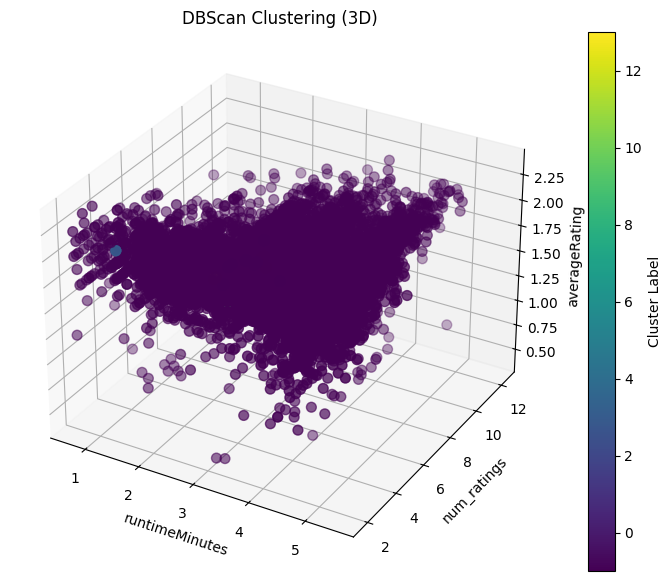
\includegraphics[width=0.4\linewidth]{3d_Dbscan.png}
    \caption{An example of the DBScan application on the dataset with standard scaling and logarithmic transformation}
    \label{fig:3d_Dbscan}
\end{figure}

\subsubsection{HDBScan}

Since DBSCAN yielded unsatisfactory results, we extended our analysis to include HDBSCAN, a more advanced density-based clustering algorithm. HDBSCAN is designed to handle datasets with clusters of varying density and can automatically determine the number of clusters. The aim was to assess whether a more flexible approach could better capture underlying structures in our data.

\begin{table}[ht!]
    \centering
    \begin{tabular}{|c|c|}
    \hline
    \multicolumn{2}{|c|}{HDBScan Clustering Results} \\
    \hline
     Preprocessing & Silhouette Score \\
    \hline
    MinMax & -0.16 \\
    MinMax \& Log & -0.05 \\
    Standard Scaling & -0.17 \\
    Standard \& Log & 0.05 \\
    \hline
    \end{tabular}
    \caption{HDBScan Clustering Results}
    \label{table:HDB}
\end{table}
However, as shown in Table \ref{table:HDB}, the silhouette scores remain low across all preprocessing variants, confirming that our dataset does not exhibit the kind of density-based structure that these algorithms rely on.

\subsection{Agglomerative Clustering} 
Hierarchical clustering was applied using four different linkage criteria: \textit{complete linkage}, \textit{single linkage} , \textit{group average}, and \textit{Ward’s method}. Initially, the clustering was performed without a connectivity constraint; however, upon further analysis, incorporating the constraint led to more coherent and better-separated clusters, as reflected in improved silhouette scores.\newline
To evaluate the optimal number of clusters, we tested a range of values for \textit{k}, from 2 to 10, and monitored the corresponding silhouette scores to assess clustering quality. The analysis revealed a consistent trend across all linkage methods: after reaching three clusters, there was a notable decline in silhouette scores — dropping from approximately 0.60 to around 0.10. This pattern suggests that increasing the number of clusters beyond three leads to partitions that are less meaningful and less well-separated, according to the internal validation metrics. \newline
These findings indicate that hierarchical clustering can provide moderately strong results when configured carefully, but the data’s structure likely supports only a limited number of distinct clusters.

\begin{table}[ht!]
    \centering
    \begin{tabular}{|c|c|c|}
    \hline
    \multicolumn{3}{|c|}{Hierarchical Clustering Results} \\
    \hline
    Preprocessing & Algorithm & Silhouette Score \\
    \hline
    MinMax & Average Link & 0.70 \\
    MinMax \& Log & Average Link & 0.50 \\
    Standard Scaling & Complete Linkage & 0.92 \\
    Standard \& Log & Average Linkage & 0.71 \\
    \hline
    \end{tabular}
    \caption{Hierarchical Clustering Results}
    \label{table:Agg_Clustering}
\end{table}
Table \ref{table:Agg_Clustering} summarizes the best silhouette scores achieved across the different hierarchical clustering methods and preprocessing techniques. \newline
Although the silhouette scores initially appeared promising, further visual inspection revealed that the resulting clusters do not reflect meaningful groupings within the data. Specifically, all hierarchical clustering configurations — regardless of linkage method or preprocessing — produced one dominant cluster containing the vast majority of instances, and a few very small clusters with little to no data points. \newline
This pattern is illustrated in the figures below. In each case, the clustering results are heavily imbalanced, with poor separation between clusters. As a result, despite seemingly good silhouette values in some cases, the clusters lack interpretability and real-world relevance, suggesting that hierarchical clustering is not well-suited to this dataset.
\begin{figure}[ht!]
    \centering
    \begin{subfigure}[b]{0.45\textwidth}
        \centering
        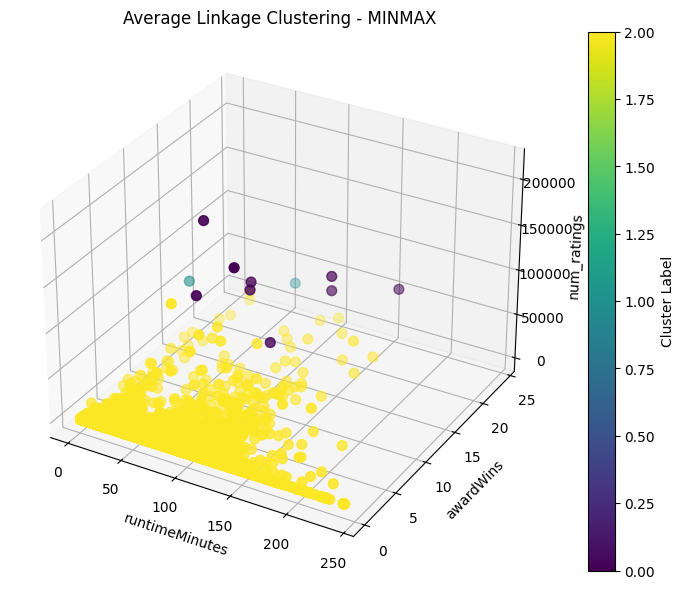
\includegraphics[width=\textwidth]{avglink_minmax.png}
        \caption{Average Linkage on MinMax Scaled Data}
        \label{fig:img1}
    \end{subfigure}
    \hfill
    \begin{subfigure}[b]{0.45\textwidth}
        \centering
        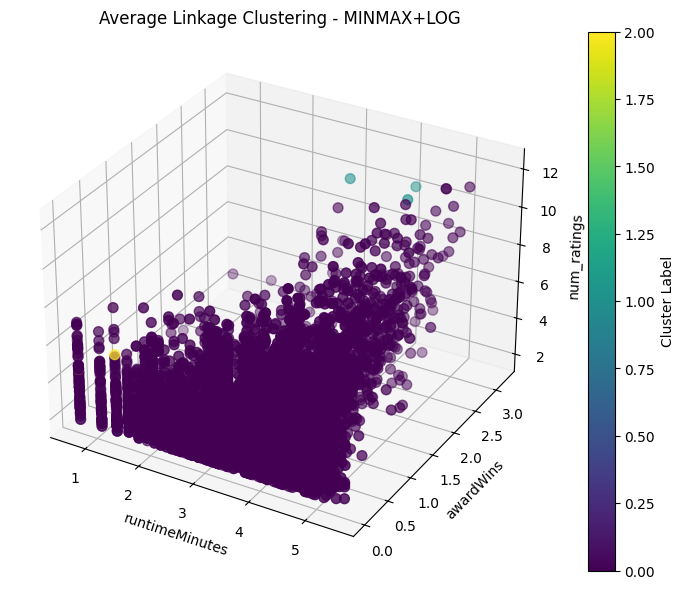
\includegraphics[width=\textwidth]{avglink_minmaxlog.png}
        \caption{Average Linkage on MinMax Scaled + Log Transformed Data}
        \label{fig:img2}
    \end{subfigure}
    \caption{Comparison of clustering results on MinMax-scaled datasets}
    \label{fig:confronto_MinMax}
\end{figure}

\begin{figure}[ht!]
    \centering
    \begin{subfigure}[b]{0.45\textwidth}
        \centering
        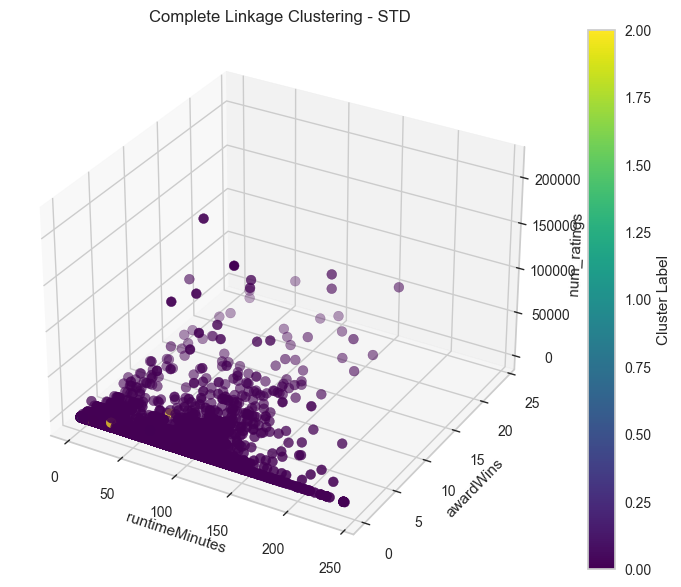
\includegraphics[width=\textwidth]{complink_std.png}
        \caption{Complete Linkage on Standard Scaled Data}
        \label{fig:img3}
    \end{subfigure}
    \hfill
    \begin{subfigure}[b]{0.45\textwidth}
        \centering
        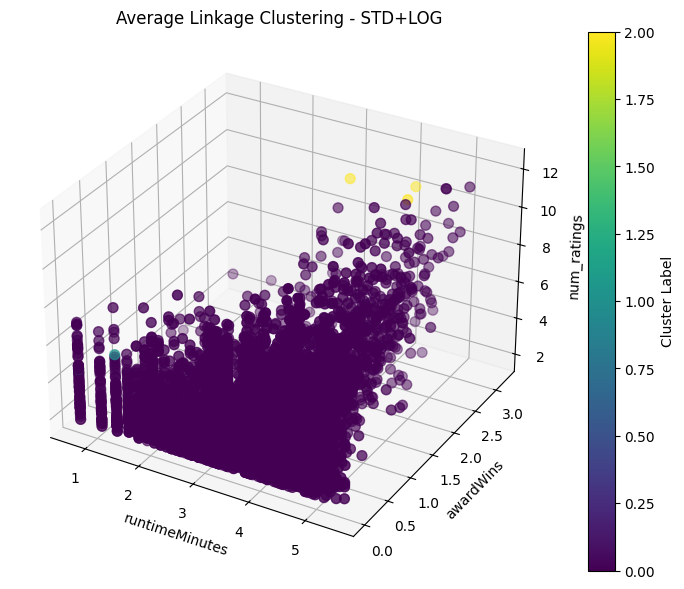
\includegraphics[width=\textwidth]{avglink_STDLOG.png}
        \caption{Average Linkage on Standard Scaled + Log Transformed Data}
        \label{fig:img4}
    \end{subfigure}
    \caption{Comparison of clustering results on Standard-scaled datasets}
    \label{fig:confronto_STD}
\end{figure}

\subsection{Discussion of the results}
The most meaningful partition was achieved using KMeans on the MinMax-scaled dataset. Although this method did not yield the highest silhouette score, as previously discussed, a higher silhouette score did not consistently result in more interpretable or useful clustering within our dataset. Therefore, we selected this configuration for a deeper interpretative analysis.
Our initial focus was on understanding how KMeans utilizes the available features, as visualized in Figure \ref{fig:km_f}
\begin{figure}[ht!]
    \centering
    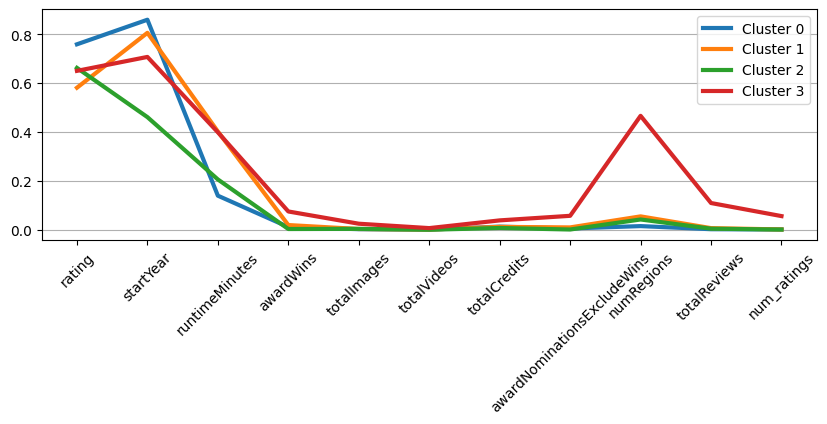
\includegraphics[width=0.4\linewidth]{kmeans_features.png}
    \caption{Feature usage by KMeans clustering}
    \label{fig:km_f}
\end{figure}

As shown, KMeans places more emphasis on certain features, while largely ignoring others. Notably, features such as\texttt{awardWins}, \texttt{totalImages}, \texttt{totalVideos} and \texttt{totalCredits} appear to contribute less to the clustering process. This is consistent with their distribution in the dataset: they are sparse and dominated by zero values, with only occasional peaks, making them less informative overall.
\begin{figure}[ht!]
        \centering
        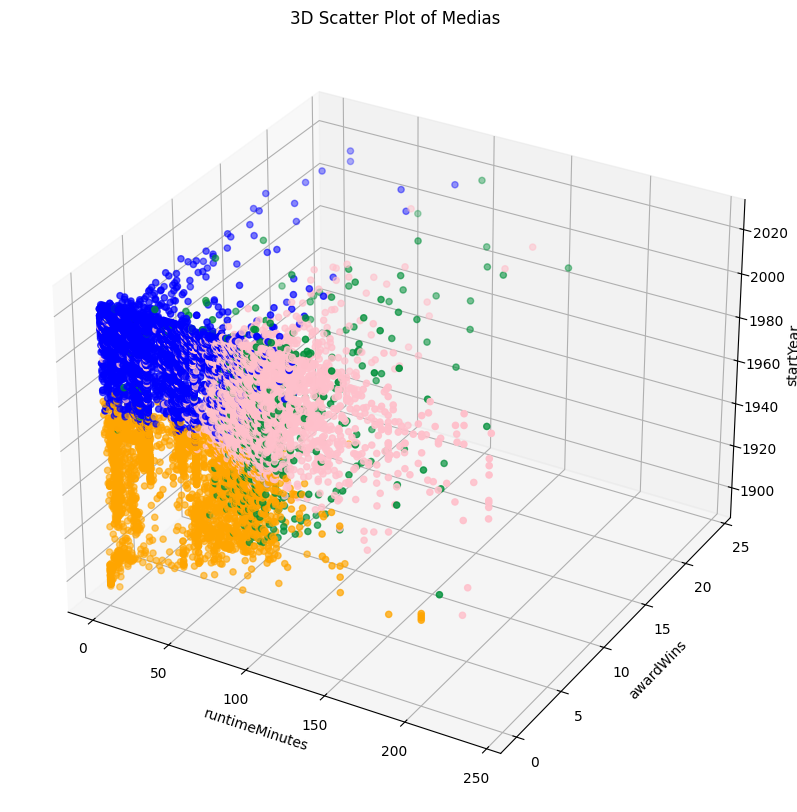
\includegraphics[width=0.4\linewidth]{3d_kmeans.png}
        \caption{3d Scatter Plot of the KMeans clusters}
        \label{fig:3d_km}
\end{figure}

To better understand the spatial distribution of the resulting clusters, a 3D scatter plot was generated using three of the most informative features:  \texttt{runtimeMinutes}, \texttt{awardWins} and \texttt{startYear} (Figure \ref{fig:3d_km}).

The clusters appear tightly grouped with significant overlap, showing no strong visual separation in feature space. Nevertheless, some semantic distinctions can still be inferred:
\begin{itemize}
    \item\textbf{Orange cluster}: composed of heterogeneous products with low \texttt{awardWins},and generally older \texttt{startYear} values. These items are likely forgotten or less popular older media, as this group was also associated with low numbers of ratings in earlier analyses.
    \item\textbf{Green cluster}: also primarily older products, but with more variation in length and higher \texttt{awardWins}. This group likely represents critically acclaimed older media, distinguishing itself from the orange cluster in terms of critical reception.
    \item\textbf{Blue cluster}: contains mostly newer, shorter productions with a broad range of \texttt{awardWins}. It can be interpreted as representing modern television and short-format productions with mixed reception. 
    \item\textbf{Pink cluster}: characterized by longer runtimes, likely indicating films or feature-length content. These products are mostly recent and include both highly acclaimed works and those with fewer awards, suggesting a general grouping of newer movies and long-form media.
\end{itemize}
To support these interpretations, Figure \ref{fig:distrib_knn} shows the distribution of titleType across the clusters:
\begin{figure}[ht!]
        \centering
        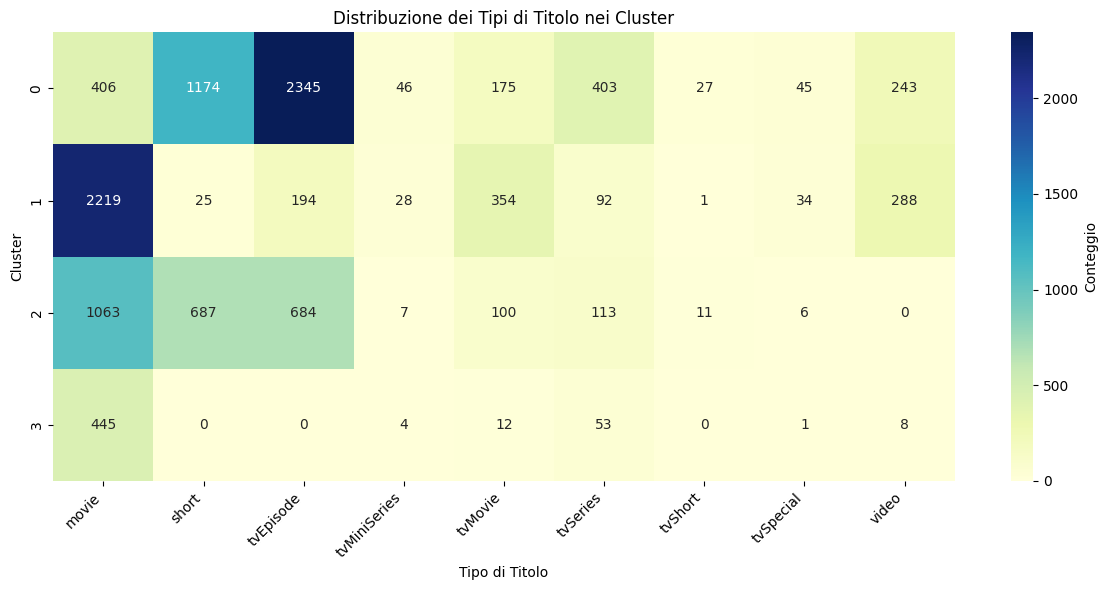
\includegraphics[width=0.4\linewidth]{distribution_kn.png}
        \caption{Distribution of the title types in the different clusters}
        \label{fig:distrib_knn}
\end{figure}

\section{Classification}
Classification is a supervised machine learning technique used to predict categorical outcomes. It involves training a model on labeled data, where each instance is associated with a known class. The model learns to recognize patterns from this training data and is then able to classify new, unseen inputs into predefined categories. \newline
For our classification task, we experimented with three supervised learning algorithms: K-Nearest Neighbors (KNN), Naive Bayes, and Decision Tree. The goal was to predict the type of media product based on various features, with the target variable being \texttt{titleType}. Each model was trained on a designated training set and evaluated on a separate test set.

\subsection{Data preparation}
To ensure consistency and comparability across classifiers, we used a common dataset for all models. However, specific preprocessing steps were applied where appropriate to optimize performance. \newline
The features selected for model training were: \texttt{AwardWins}, \texttt{\seqsplit{awardNominationsExcludeWins}}, \texttt{numRegion}, \texttt{genres}, \texttt{TotalReviews}, \texttt{decade}, \texttt{continent}, \texttt{rating\_category}, \texttt{popularity\_category}, \newline
\texttt{\seqsplit{runtime\_category}}

The last three — rating\_category, popularity\_category, and runtime\_category — were derived by binning the original continuous variables: rating, num\_rating, and runtimeMinutes respectively. The remaining numeric features were normalized using a logarithmic transformation followed by MinMax scaling to ensure all input values were on a comparable scale. \newline
The target variable, titleType, was refined to focus on cinema and television products. We excluded categories such as video games, and merged several low-frequency or similar TV-related categories (tvMiniSeries, tvSpecial, and tvShort) into a consolidated class labeled otherTvProducts. This decision was made to address class imbalance and improve the generalizability of our models.

\subsection{KNN}
The first model applied was the K-Nearest Neighbors (KNN) algorithm, a non-parametric supervised learning method that classifies data points based on the majority class among their \textit{k} nearest neighbors in the training set. KNN makes no assumptions about the underlying data distribution and is particularly effective in cases where similar instances belong to the same class. \newline
To optimize model performance, we employed GridSearch to determine the best hyperparameters. The optimal configuration was:
\begin{itemize}
    \item \textbf{Distance metric} =\texttt{cityblock}
    \item \textbf{Number of neighbors (k)} = 5
    \item \textbf{Weights strategy} =\texttt{distance}
\end{itemize}
Given the presence of class imbalance in the dataset, we selected balanced accuracy as the primary scoring metric during hyperparameter tuning. The model achieved an accuracy score of 0.76 on the training set. \newline
While accuracy is easy to interpret, it may not reflect true model performance in the presence of class imbalance. For this reason, we also evaluated the model using precision, recall, and the F1-score for a more balanced perspective.
\begin{figure}[ht]
    \centering
    \begin{minipage}{0.48\textwidth}
        \centering
        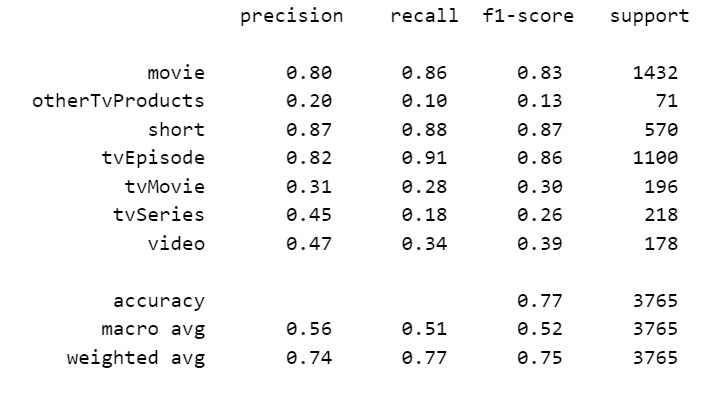
\includegraphics[width=\linewidth]{Report_knn.png}
        \caption{KNN Classification Report}
        \label{fig:knn_report}
    \end{minipage}
    \hfill
    \begin{minipage}{0.48\textwidth}
        \centering
        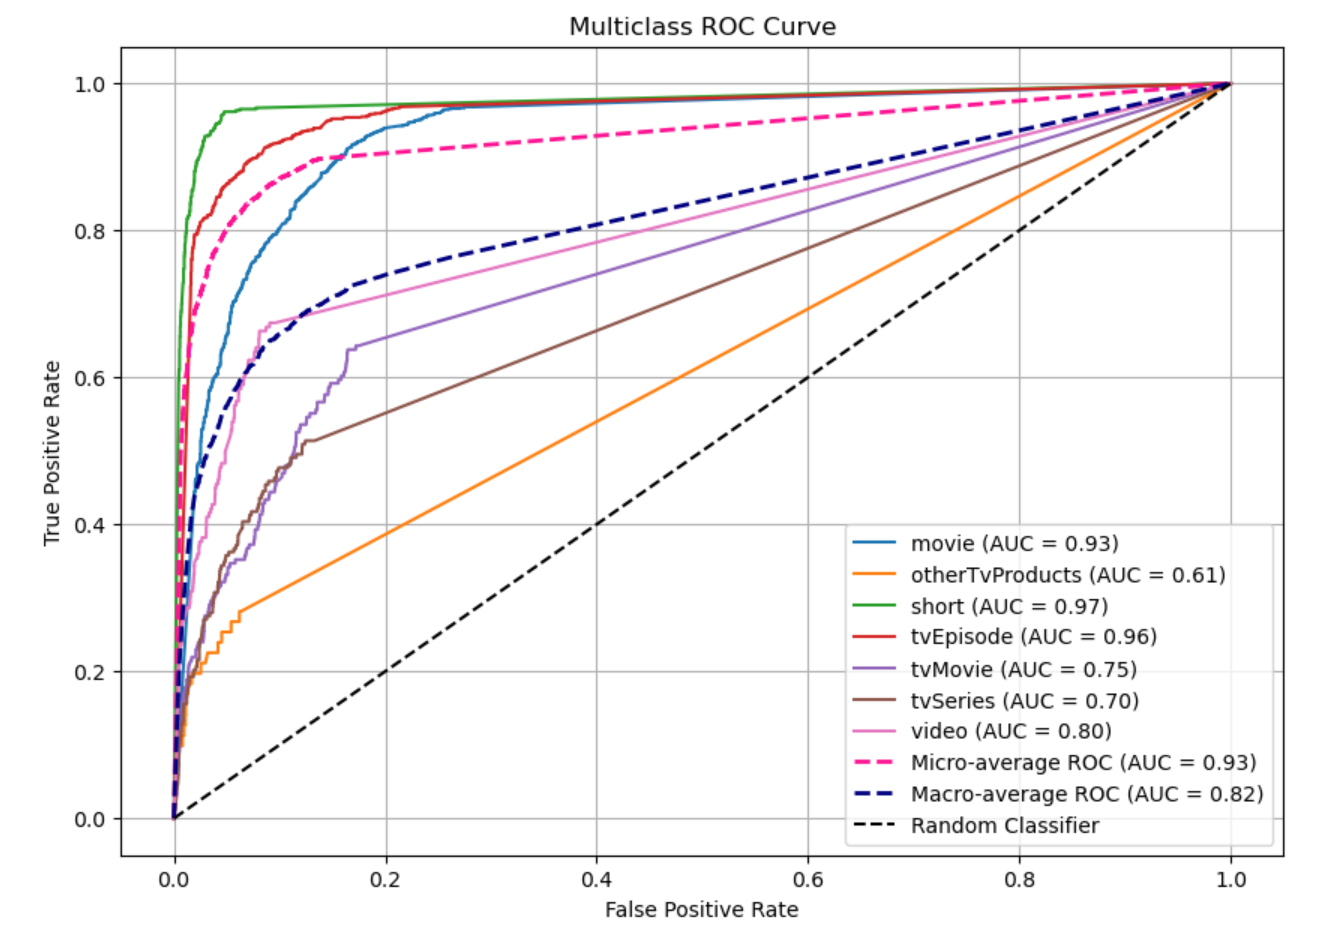
\includegraphics[width=\linewidth]{rocknn.png}
        \caption{KNN ROC Curve}
        \label{fig:knn_roc}
    \end{minipage}
\end{figure}
As shown in Figure \ref{fig:knn_report}, model performance varies across classes, which is expected due to the unequal distribution of samples. Despite this, the model achieved a solid accuracy of 0.77 on the test set, indicating good overall performance. \newline
The ROC curves in Figure \ref{fig:knn_roc} display, for each class, the trade-off between the True Positive Rate (TPR) — the proportion of actual positives correctly predicted — and the False Positive Rate (FPR) — the proportion of negatives incorrectly predicted as positives. This visualization is particularly valuable in multiclass classification tasks, as it reveals how well the model distinguishes each class from the rest.\newline
On average, the model demonstrated a high TPR-to-FPR ratio of 0.88, suggesting that it is able to reliably identify the correct class in most cases. This indicates that the KNN classifier performs robustly across the diverse categories in the dataset, especially when using the tuned hyperparameters and an appropriate distance metric.

\subsection{Naïve Bayes}
In this section, we examine the performance of our model using the Naïve Bayes classifier, a probabilistic approach grounded in Bayesian statistics. Naïve Bayes refers to a family of simple algorithms for constructing classifiers—models that assign class labels to instances represented as vectors of feature values, with labels drawn from a finite set of categories. \newline
While there is no single algorithm that defines all Naïve Bayes classifiers, they are unified by a key assumption: that the value of each feature is conditionally independent of the others, given the class label. This simplifying assumption forms the core of the model and enables efficient computation of class probabilities.

\begin{figure}[ht]
    \centering
    \begin{minipage}{0.48\textwidth}
        \centering
        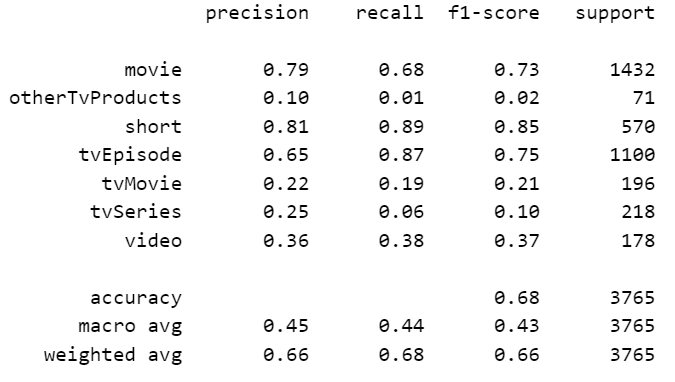
\includegraphics[width=\linewidth]{Report_naiveB.png}
        \caption{Naïve Bayes Classification Report}
        \label{fig:nb_report}
    \end{minipage}
    \hfill
    \begin{minipage}{0.48\textwidth}
        \centering
        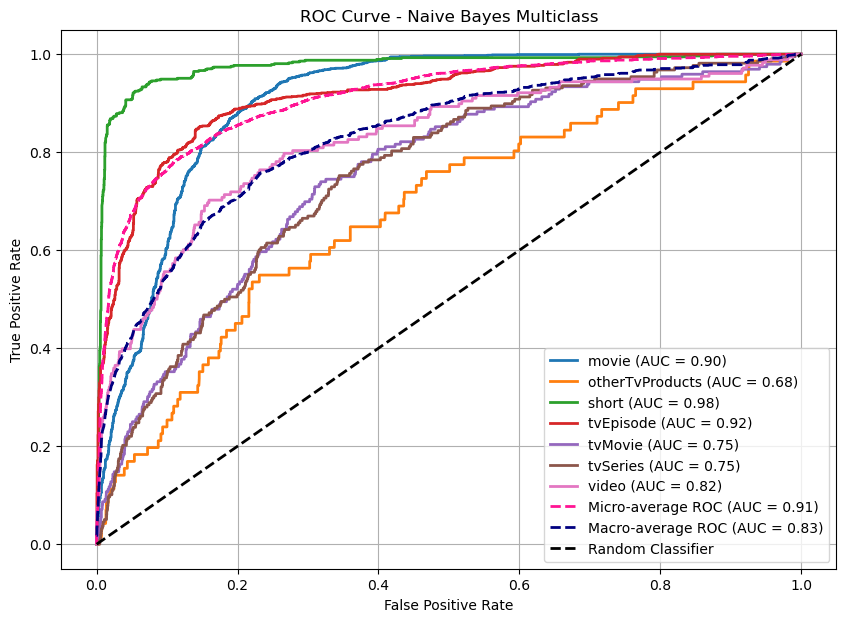
\includegraphics[width=\linewidth]{rocnb.png}
        \caption{ Naïve Bayes ROC Curve}
        \label{fig:nb_roc}
   \end{minipage}
\end{figure}
We trained our model using the Multinomial Naïve Bayes algorithm and obtained the evaluation results shown in Figure \ref{fig:nb_report}. The model achieved an accuracy of 0.68 on the test set. Among all classes, the \textit{"short"} category was the easiest to predict, consistent with the results from the KNN classifier, achieving an F1-score of 85\%. \newline
Some other classes were not predicted as well; for example, certain categories had F1-scores as low as 0.01 and recall values around 0.02, indicating that the classifier struggled to correctly identify instances from those categories. \newline
The ROC curve shown in Figure \ref{fig:nb_roc} illustrates the model's performance across all classes using a one-vs-rest approach. The curves are generally plotted near the top-left corner, suggesting reasonable discriminative power.\newline
In conclusion, while the Naïve Bayes classifier performed adequately, it did not reach the accuracy level obtained with the KNN algorithm.

\subsection{Decision Tree}
A compelling alternative to probabilistic models like Naïve Bayes and instance-based approaches such as KNN is the Decision Tree classifier. This non-parametric, supervised learning method is particularly valued for its interpretability and ability to model complex decision boundaries without requiring feature scaling. \newline
A Decision Tree builds a hierarchical structure by recursively partitioning the dataset based on feature values, aiming to create subsets that are increasingly homogeneous with respect to the target label. It comprises:
\begin{itemize}
	\item Internal nodes, which test specific feature values.
	\item Branches, representing the outcome of a those tests.
	\item Leaf nodes, which assign a final class label 
\end{itemize}
To fine-tune the model and control its complexity, we focused on three critical hyperparameters: \texttt{min\_samples\_split}, \texttt{min\_samples\_leaf}, \texttt{max\_depth}. Using Randomized Search, we identified the optimal configuration as follows:
\begin{itemize}
    \item \texttt{min\_samples\_split} = 96
    \item \texttt{min\_samples\_leaf} = 31
    \item \texttt{max\_depth} = 12
\end{itemize}
The splitting criterion selected was the Gini index, which measures node impurity and helps separate target classes effectively. To improve generalization and reduce overfitting, we applied Cost-Complexity Pruning (CCP), which simplifies the tree by removing branches with little predictive power. The pruning parameter $\alpha$ controls the trade-off between complexity and accuracy: higher values lead to simpler models, while lower values retain complexity but risk overfitting. Our optimal $\alpha$ was 0.00103, indicating a relatively low level of pruning and a balanced model. \newline
On the training set, accuracy improved slightly by 0.02\%, from 0.62 to 0.64. Using the best parameters found via Randomized Search and the selected $\alpha$, the Decision Tree achieved an accuracy of 0.64 on the test set. 
\begin{figure}[ht]
    \centering
    \begin{minipage}{0.48\textwidth}
        \centering
        \includegraphics[width=\linewidth]{Dt_reportval.png}
        \caption{Decision Tree Classification Report on train set}
        \label{fig:dt_report}
    \end{minipage}
    \hfill
    \begin{minipage}{0.48\textwidth}
        \centering
        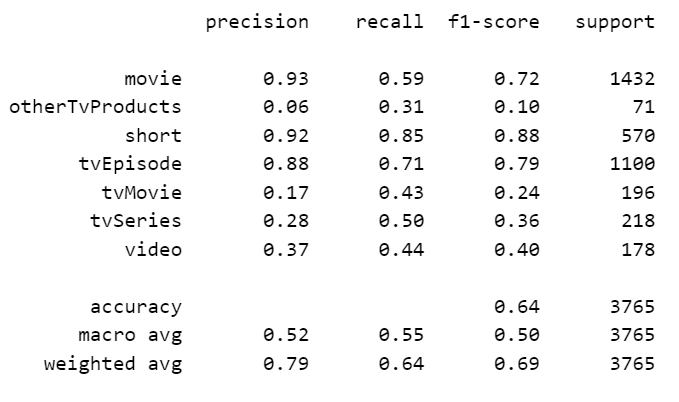
\includegraphics[width=\linewidth]{ReportDT.png}
        \caption{Decision Tree Classification Report on test set}
        \label{fig:dt_report}
    \end{minipage}
\end{figure}
Figure \ref{fig:dt_roc} shows the ROC curve, which is consistently high across genres, indicating good discrimination between classes. The Precision-Recall curve, more informative for imbalanced datasets, reports a micro-average precision (AP) of 0.72, reflecting strong overall performance, while the macro-average AP of 0.52 indicates weaker performance on minority classes. This difference arises because the ROC curve is less sensitive to class imbalance, calculating TPR and FPR over all instances regardless of class distribution, whereas the Precision-Recall curve provides a more meaningful evaluation in imbalanced scenarios.
\begin{figure}[ht]
    \centering
    \begin{minipage}{0.48\textwidth}
        \centering
        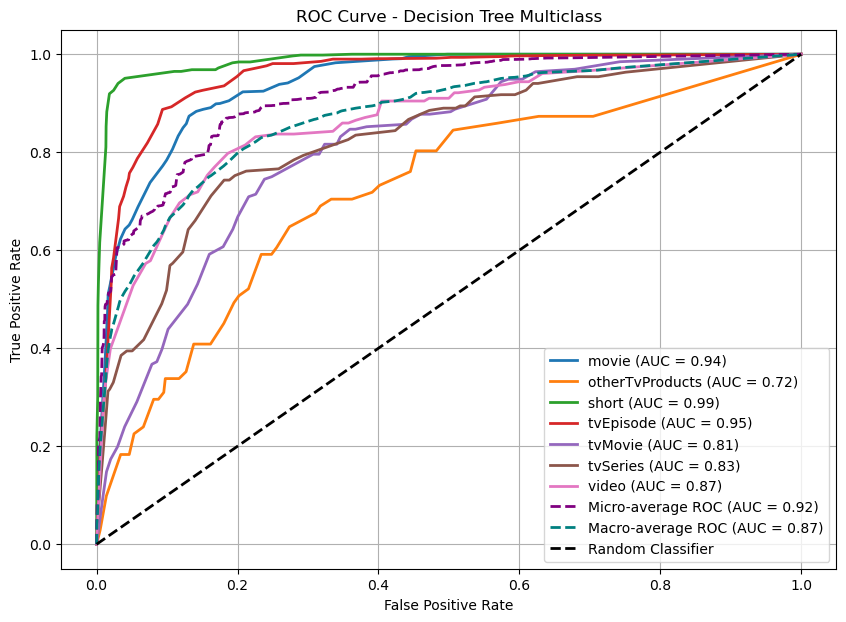
\includegraphics[width=\linewidth]{RocDT.png}
        \caption{Decision Tree Roc Curve}
        \label{fig:dt_roc}
    \end{minipage}
    \hfill
    \begin{minipage}{0.48\textwidth}
        \centering
        \includegraphics[width=\linewidth]{RecallDT.png}
        \caption{Decision Tree Precision-Recall curve}
        \label{fig:dt_pr}
    \end{minipage}
\end{figure}
\subsection{Classification conclusion}
After evaluating the results of each classification algorithm, we concluded that the K-Nearest Neighbors (KNN) classifier delivered the best performance, achieving an accuracy score of 0.77, followed by the Naïve Bayes classifier with an accuracy of 0.68.
\section{Regression}
For this task two datasets were used, as for classification: the training and the test datasets resulting from the preprocessing phase. Additional preprocessing was applied to both datasets. \newline
Since regression is the task of predicting a continue numerical feature, all non-numerical and categorical columns were dropped, resulting in the following ones: \texttt{num\_ratings}, \texttt{startYear}, \texttt{runtimeMinutes}, \texttt{awardWins}, \texttt{totalImages}, \texttt{totalVideo}, \texttt{totalCredits}, \texttt{\seqsplit{awardNominationsExcludeWins}}, \texttt{numRegions}, \texttt{totalReviews}.

The analysis focused on multivariate regression, at first with just one target variable for which we used a \textit{Linear Regressor} and a \textit{Decision Tree Regressor}, and then multivariate regression with two target variables, using again a \textit{Decision Tree Regressor}.
The variables normalized with MinMax scaling and the logarithmic transformation were used just for the \textit{Linear Regressor}, meanwhile for the \textit{Decision Trees} we kept them as they were to preserve the interpretability of the model. This was done with the second part of the analysis in mind, which is to understand whether the most important features selected by the multivariate-single target \textit{Decision Tree} were useful to better the performance of the \textit{Linear Regressor}. \newline
A dummy regressor was also trained as a tool of comparison, with the \textit{strategy} parameter set to \textit{mean}. The R2 value obtained was of -0.00027 which can be approximated as 0.

\subsection{Results of the Multivariate Regression with One Target Variable}
The target variable chosen to be predicted in the multivariate-single target scenario was the one deemed most interesting to be used, the \textit{rating} variable: this is because predicting the rating of a media could potentially mean being able to predict its success.
The Linear Regressor which used all the variables available had the worst performance overall, not even surpassing the dummy classifier. This was probabily because of a lack of linear relationships in the data and possibly a number of features which was too high and not informative. In table \ref{table:lr_results}, the results:

\begin{table}[h]
    \centering
    \begin{tabular}{|c|c|c|}
    \hline
    \multicolumn{3}{|c|}{Linear Regressor Results} \\
    \hline
    MSE & MAE & R2 \\
    \hline
    0.44 & 0.65 & -19.7 \\
    \hline
    \end{tabular}
    \caption{Linear Regressor Results}
    \label{table:lr_results}
\end{table}

In image \ref{fig:linear_scatterplot}, the relationship between the actual rating, the predicted rating and the number of awardWins is shown: it can be seen how the linear regressor always predicts the same value for all instances.

\begin{figure}[h!]
    \centering
    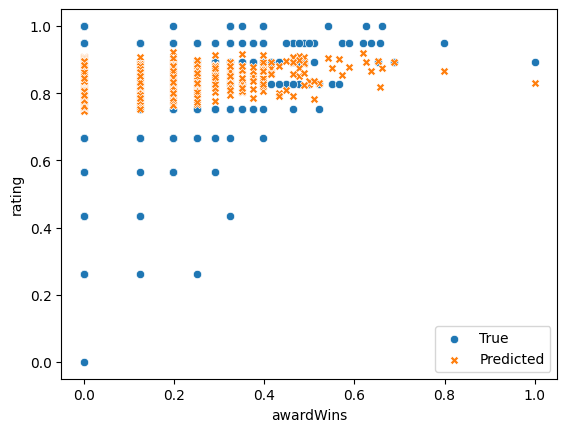
\includegraphics[width=0.4\linewidth]{linear_scatterplot.png}
    \caption{Scatterplot showing behaviour of Linear Regressor}
    \label{fig:linear_scatterplot}
\end{figure}

As for the Decision Tree used for the multivariate-single target regression, the performance was better than the one of both the \textit{Dummy Classifier} and the \textit{Linear Regressor}. The model was trained using a Grid Search using 10 folds and otpimizing the following parameters: \textit{criterion}, \textit{min\_samples\_split},\textit{min\_sample\_leaf}, \textit{max\_depth} and \textit{ccp\_alpha}. The best values were found to be, respectively: squared\_error, 3, 5, 6 and 0.00.
The results obtained were:
\begin{itemize}
    \item R2: 0.191
    \item MSE: 1.558
    \item MAE: 0.950
\end{itemize}

In figure \ref{fig:tree_plot}, the first tree levels of the Decision Tree plotted: 

\begin{figure}[h]
    \centering
    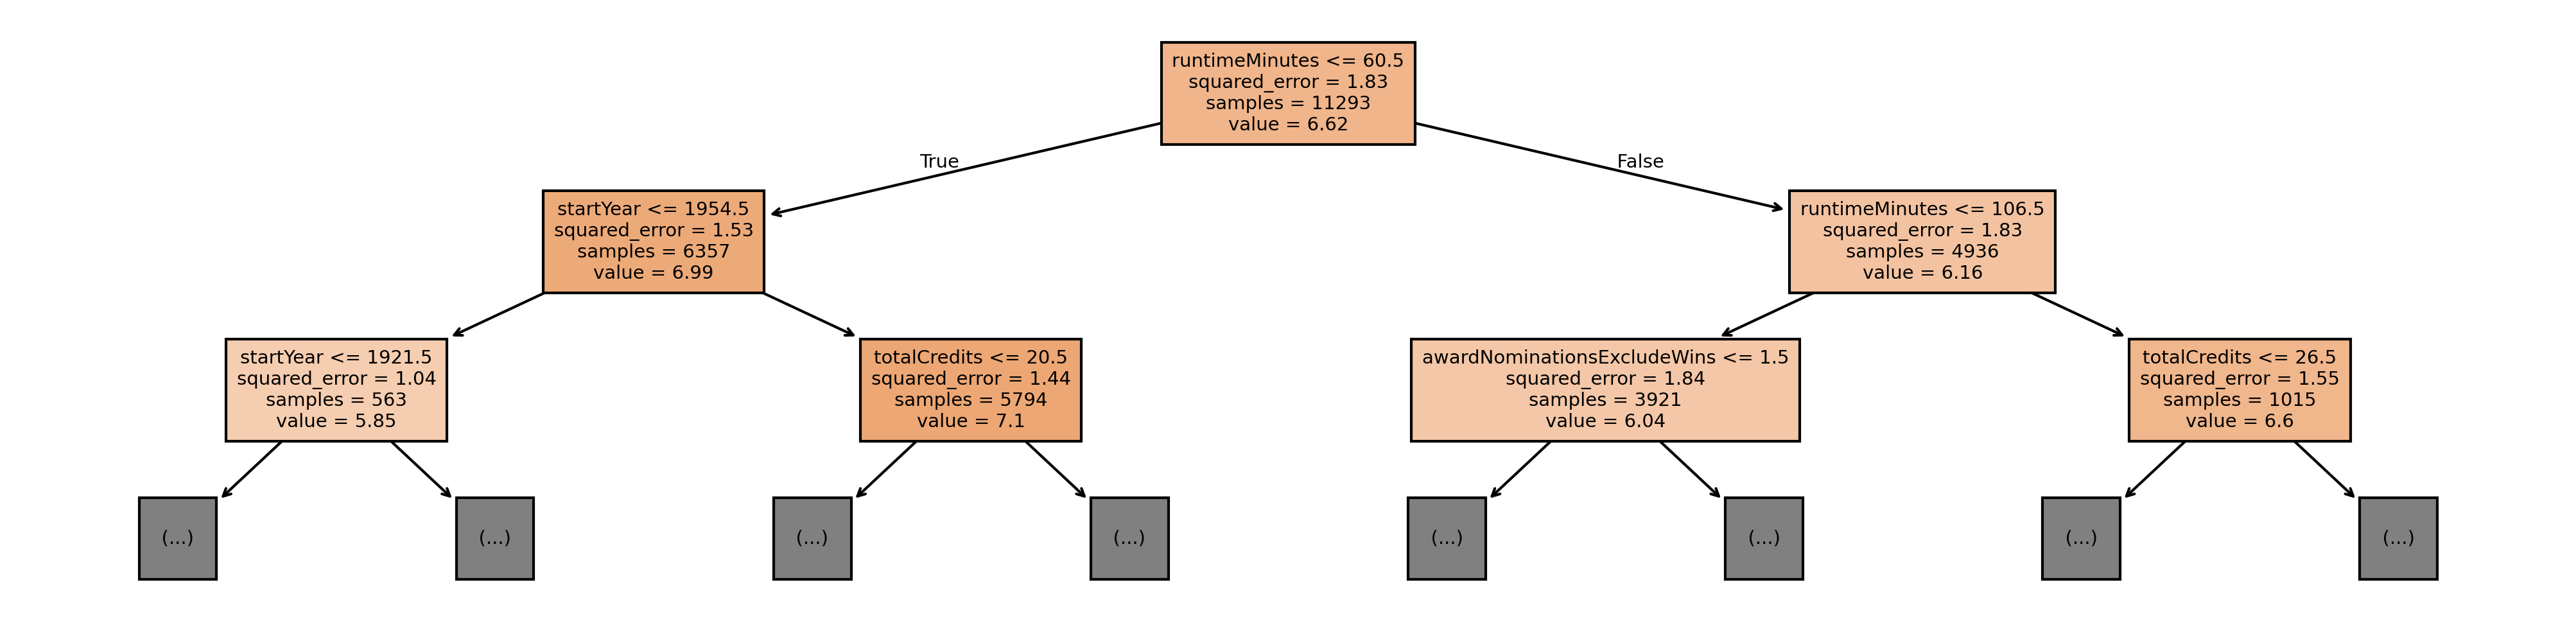
\includegraphics[width=0.4\linewidth]{tree_plot.png}
    \caption{Plot of the Decision Tree - Multivariate \& Single Variable}
    \label{fig:tree_plot}
\end{figure}

\subsection{Feature Importances for the Linear Regressor}
To perform this second part of the analysis, the first action made was to print out the feature importances of the \textit{Decision Tree Regressor} (DTR). Many trials were conducted to understand how many of the features found by the DTR were most meaningful for the \textit{Linear Regressor}, finding the following were most helpful: \texttt{runtimeMinutes}, \texttt{startYear}, \texttt{num\_ratings}, \texttt{totalCredits}, \texttt{numRegions}. \newline
Overall, the Linear Regressor performance is still not good, but it did get significantly better, as shown in table \ref{table:lr_fi}:

\begin{table}[h]
    \centering
    \begin{tabular}{|c|c|c|}
    \hline
    \multicolumn{3}{|c|}{Linear Regressor with Feature Importance} \\
    \hline
    MSE & MAE & R\^2 \\
    \hline
    0.0106 & 0.073 & 0.0526 \\
    \hline
    \end{tabular}
    \caption{Linear Regressor with Feature Importance}
    \label{table:lr_fi}
\end{table}

\subsection{Results of the Multivariate Regression with Two Target Variables}
This analysis was performed using again a Decision Tree Regressor, which was optimized using a grid search over the same parameter's grid that was used before. This time, the best parameters found were: as for criterion it was absolute error, the \texttt{ccp\_alpha} was 0.01,  \texttt{the max\_depth} was best at None, and the  \texttt{min\_samples\_leaf} and  \texttt{min\_samples\_split} were respectively at 5 and 3. \\
As dependent variables  \texttt{rating} and  \texttt{num\_ratings} were chosen, to continue on the path of predicting the possibile popularity of a product. In table \ref{table:dt_2t} the results:

\begin{table}[h]
    \centering
    \begin{tabular}{|c|c|c|}
    \hline
    \multicolumn{3}{|c|}{Decision Tree-Multivariate Regression with 2 Targets} \\
    \hline
    MSE & MAE & $R^2$ \\
    \hline
    156525714.8 & 461.503 & 0.228 \\
    \hline
    \end{tabular}
    \caption{Decision Tree-Multivariate Regression with 2 Targets}
    \label{table:dt_2t}
\end{table}

Although the $R^2$ is at the highest, the MSE and the MAE are also at their highest, signaling that the model is able to understand some variance in the data but is not capable of predicting the instances properly.

\section{Pattern Mining}
\subsection{Data Preparation}

The \textbf{data preparation} phase for pattern mining was carried out with the aim of selecting and processing only the most semantically relevant features, in order to extract interpretable patterns.
Following an initial exploratory inspection, variables considered uninformative or redundant for the analysis—such as \texttt{originalTitle}, \texttt{totalImages}, \texttt{totalVideos}, \texttt{totalCredits}, and \texttt{canHaveEpisodes}—were removed. Additionally, the \texttt{short} label from the \texttt{titleType} feature was discarded, as this information was already represented in the \texttt{genres} attribute.

\paragraph{Categorical feature processing.}
To reduce the cardinality and asymmetry of the \texttt{countryOfOrigin} feature, a new variable \texttt{continent} was introduced via ISO mapping using the \texttt{pycountry} library. Countries that could not be mapped to a known continent (tagged as \texttt{Unknown}) were excluded to ensure semantic consistency.  
The \texttt{continent} and \texttt{genres} features, being multi-label in nature, were transformed into binary format using the \texttt{MultiLabelBinarizer} class, generating a set of binary columns with coherent prefixes (e.g., \texttt{genre\_Comedy}, \texttt{continent\_Europe}).  
The \texttt{titleType} feature was instead encoded using \texttt{get\_dummies}, producing a standard one-hot representation.

\paragraph{Transformation of numerical variables.}
A mixed approach was adopted for the numerical features, based on discretization techniques guided by empirical distributions and clustering.
The \texttt{num\_ratings} variable, which was highly skewed, was transformed using a logarithmic function (\texttt{log1p}) and subsequently standardized via \texttt{MinMaxScaler}. It was then discretized using \texttt{KMeans} clustering (\texttt{k=5}). The resulting clusters were ordered based on the median and renamed according to rating volume (\texttt{Very Low} -- \texttt{Very High}).

\begin{figure}[H]
    \centering
    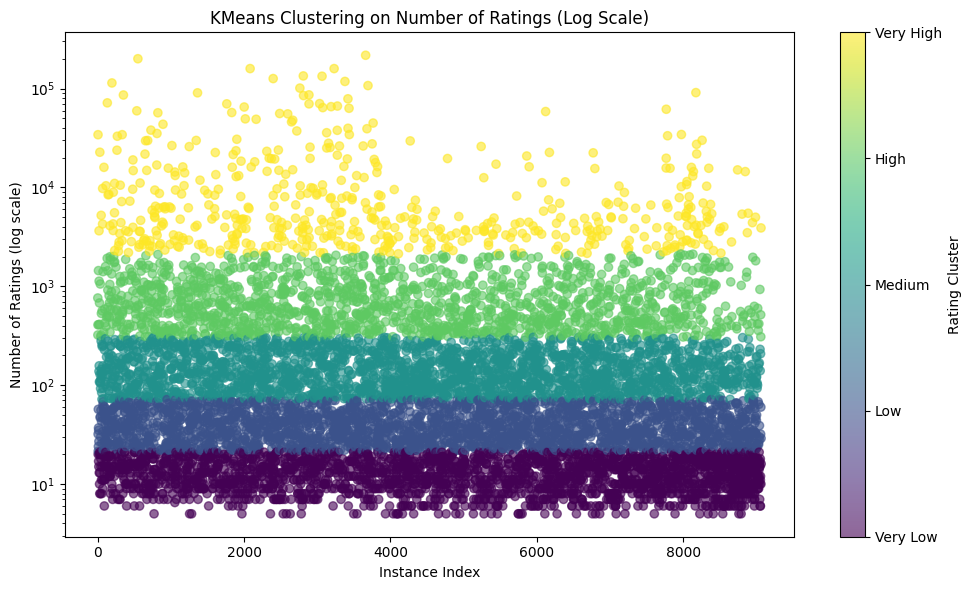
\includegraphics[width=0.4\linewidth]{Kmeans_num_rating.png}
    \caption{Scatterplot K-Means num\_ratings}
    \label{fig:enter-label}
\end{figure}


\paragraph{Definition of the \texttt{success\_class} variable.}

Since the dataset did not contain a direct measure of critical recognition, the target variable \texttt{success\_class} was constructed using a rule-based logic that incorporates both critical reviews and award-related information. In particular:
\begin{itemize}
  \item A title is labeled as \texttt{Critically Acclaimed} if it has received at least one award or one nomination;
  \item If it has not received awards or nominations but has at least one critical review, it is labeled as \texttt{Considered by Critics};
  \item Titles with no critical reviews and no recognition are classified as \texttt{Flop}.
\end{itemize}

\begin{table}[H]
    \centering
    \begin{tabular}{cc}
        Flop & 5022\\
        \hline
        Considered by Critics & 2466 \\
        \hline
        Critically Acclaimed & 1580\\
    \end{tabular}
    \caption{Distribution of the \texttt{success\_class} target variable in the development set based on critical reviews, awards, and nominations.}

    \label{tab:my_label}
\end{table}

\paragraph{Logical discretization of additional features.}
To improve the interpretability of the patterns, additional numerical variables were discretized using manually defined thresholds based on empirical criteria:

\begin{itemize}
  \item \texttt{numRegions}: \texttt{Local} if equal to 1, \texttt{Limited} if $\leq$5, \texttt{Moderate} if $\leq$10, and \texttt{International} otherwise;
  \item \texttt{rating}: \texttt{Poor} (0--5), \texttt{Average} (5--6.5), \texttt{Good} (6.5--7.5), \texttt{Excellent} ($>$7.5);
\item \texttt{runtimeMinutes}: discretized into \texttt{Short} ($\leq$60 min), \texttt{Standard} (61–90 min), \texttt{Long} (91–120 min), \texttt{Extended} (121–150 min), and \texttt{Epic} ($>$150 min) based on fixed duration intervals.

\end{itemize}

\subsection{Frequent Pattern Extraction}
The \textit{Apriori} and \textit{FP-Growth} algorithms were employed with varying values of minimum support (\texttt{min\_support}) and minimum itemset cardinality (\texttt{zmin}). The trend in the number of frequent, maximal, and closed itemsets was analyzed as a function of support thresholds, highlighting the exponential growth in the number of patterns with increasing granularity.
\subsubsection{Discussion on Frequent Patterns}

The analysis was conducted on a transactional dataset obtained by transforming the categorical and binary variables of the original dataset, representing each movie as a distinct set of items.

For each parameter combination, the following were generated:
\begin{itemize}
    \item \textbf{Maximal itemsets} (\texttt{target='m'}), which cannot be further extended without reducing support;
    \item \textbf{Closed itemsets} (\texttt{target='c'}), which preserve the maximum amount of information while reducing redundancy.
\end{itemize}

The visualizations obtained reveal that the most frequent patterns are dominated by combinations of film genres, confirming the presence of well-established semantic structures within the dataset.

\begin{figure}[H]
\centering
\begin{minipage}{0.48\textwidth}
  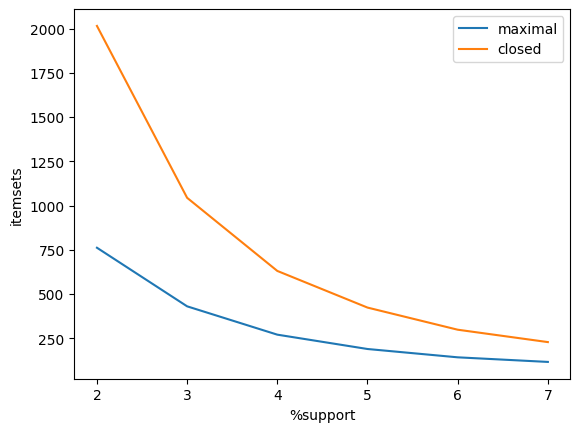
\includegraphics[width=\linewidth]{zmin2.png}
  \caption{Closed and maximal itemsets for \texttt{zmin=2}.}
  \label{fig:itemset_zmin2}
\end{minipage}
\hfill
\begin{minipage}{0.48\textwidth}
  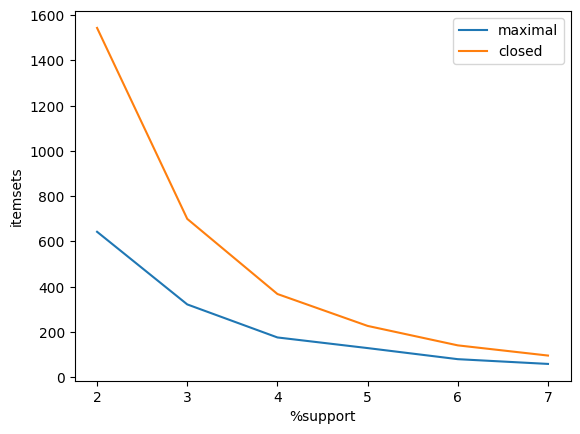
\includegraphics[width=\linewidth]{zmin3.png}
  \caption{Closed and maximal itemsets for \texttt{zmin=3}.}
  \label{fig:itemset_zmin3}
\end{minipage}
\end{figure}

As expected, increasing the support threshold leads to a significant reduction in the number of patterns. Moreover, closed itemsets consistently outnumber maximal ones, as they retain more statistical information. Raising \texttt{zmin} from 2 to 3 further decreases the number of patterns, enhancing readability at the cost of simpler pattern loss.

To compare the efficiency and productivity of the Apriori and FP-Growth algorithms, the number of itemsets generated was evaluated at different support levels and itemset sizes. The results are summarized in Table~\ref{tab:algo_comparison}.

\begin{table}[H]
\centering
\caption{Comparison between Apriori and FP-Growth across support and itemset sizes}
\label{tab:algo_comparison}
\begin{tabular}{|c|c|c|c|}
\hline
\textbf{Support (\%)} & \textbf{Itemset size} & \textbf{Apriori} & \textbf{FP-Growth} \\
\hline
8 & 2 & 170 & 113 \\
20 & 2 & 15 & 399 \\
8 & 3 & 3 & 1896 \\
20 & 3 & 64 & 176 \\
\hline
\end{tabular}
\end{table}

As observed, FP-Growth generates a significantly higher number of complex patterns (3-itemsets), particularly at lower support levels. This indicates a greater ability to explore intricate combinations, uncovering latent structures that Apriori tends to miss. In contrast, Apriori proves more efficient in detecting shorter patterns but lacks depth.
In light of these findings, FP-Growth with 8\% support and \texttt{zmin=3} was selected, as it provides an optimal balance between pattern granularity and semantic coverage, demonstrating superiority in both quantitative and qualitative terms for the purposes of this analysis.


\subsection{Association Rules Extraction}
Association rules were extracted using the FP-Growth algorithm, aimed at generating rules of the form:

\[
\text{Antecedent} \Rightarrow \text{Consequent}
\]

The rules were evaluated using three main metrics:
\begin{itemize}
  \item \textbf{Support}: the absolute or relative frequency of the rule's occurrence in the dataset;
  \item \textbf{Confidence}: the conditional probability of the consequent given the antecedent;
  \item \textbf{Lift}: the ratio between the observed confidence and the expected confidence under statistical independence.
\end{itemize}

The rules listed in Table~\ref{tab:regole_lift_alto} represent some of the most relevant patterns identified during the analysis, selected based on particularly high \textit{lift} values (greater than 2.5), indicating a strong and non-random association between antecedent and consequent.
For instance, the first rule shows that movies distributed internationally and labeled as \texttt{type\_movie} have a substantially higher likelihood of receiving a very high number of user ratings. This implies a strong relationship between distribution reach and popularity in terms of visibility and audience approval.
Another pattern highlights that internationally distributed \texttt{type\_movie} titles are often also labeled as \texttt{Critically Acclaimed}, meaning they receive positive recognition from critics. Such rules are especially relevant for predictive tasks involving the qualitative success of titles.
Various confidence thresholds were tested: with \texttt{conf = 30}, a total of 1072 rules were generated; with \texttt{conf = 40}, the number dropped to 580; and with \texttt{conf = 70}, only 101 rules remained. A threshold of \texttt{conf = 40} was ultimately selected, as it offered a good balance between quantity, semantic diversity, and rule quality. This threshold yields a manageable set of rules while maintaining sufficiently high confidence levels and often achieving lift values above 1.5, indicative of meaningful, non-trivial associations.
In fact, support, confidence, and lift were jointly analyzed to assess rule quality. Rules with high support ensure statistical robustness, while high confidence reflects strong predictive capability. However, it is the \textit{lift} that reveals the true associative strength: values significantly above 1 indicate non-random co-occurrence. For example, the rule \texttt{success\_class=Critically Acclaimed} $\Leftarrow$ \texttt{region\_distribution=International, type\_movie} presents a lift of 2.86 and a confidence of 0.50, suggesting a strong informative link between international distribution and critical recognition.

\begin{table}[H]
\centering
\label{tab:regole_flop}
\begin{tabular}{|p{4cm}|p{5.5cm}|c|c|c|}
\hline
\textbf{Consequent} & \textbf{Antecedent} & \textbf{Conf.} & \textbf{Lift} & \textbf{Support (\%)} \\
\hline
success\_class=Flop & continent\_North America, region\_distribution=Local & 0.689 & 1.24 & 21.55 \\
\hline
region\_distribution=Local & continent\_North America, success\_class=Flop & 0.787 & 1.47 & 21.55 \\
\hline
success\_class=Flop & rating\_category=Average, region\_distribution=Local & 0.749 & 1.35 & 13.52 \\
\hline
success\_class=Flop & genre\_Drama, region\_distribution=Local & 0.655 & 1.18 & 12.26 \\
\hline
region\_distribution=Local & genre\_Drama, continent\_North America, success\_class=Flop & 0.743 & 1.39 & 6.15 \\
\hline
success\_class=Flop & rating\_category=Average, continent\_North America, region\_distribution=Local & 0.721 & 1.30 & 6.89 \\
\hline
\caption{Examples of association rules with confidence $\geq$ 0.65 and relevant support}
\end{tabular}
\end{table}

\subsubsection{Discussion on Association Rules}

A relatively low confidence threshold (\texttt{$\geqslant$0.2}) was adopted to account for the strong class imbalance, as outlined in the \emph{data preparation} section. This trade-off allowed for the inclusion of rules that are predictively useful even for minority classes.

\begin{figure}[H]
\centering
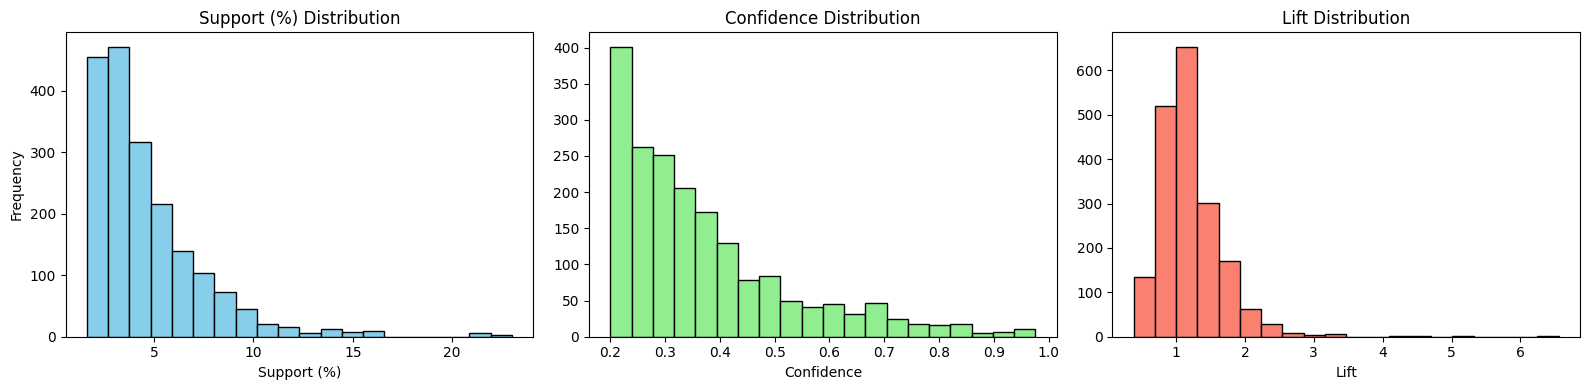
\includegraphics[width=0.4\textwidth]{dist_sup_lift_conf.png}
\caption{Distribution of association rule metrics: support, confidence, and lift}
\label{fig:metriche_regole}
\end{figure}

Figure~\ref{fig:metriche_regole} illustrates the distributions of key metrics for the association rules extracted using the FP-Growth algorithm.

\textbf{On the left}, the support distribution confirms that most rules exhibit support between 2\% and 6\%, with a steep drop beyond this range. This behavior reflects the sparse nature of the dataset, where only a few item combinations occur frequently. Rules with support above 10\% are particularly rare.

\textbf{In the center}, the confidence distribution shows a sharply decreasing trend. The majority of rules fall within the 0.2 to 0.5 confidence range, while only a minority exceed 0.7. This implies that, while many rules are statistically valid, few demonstrate strong conditional reliability.

\textbf{On the right}, the lift distribution is concentrated around 1.0, which signals statistical independence between antecedent and consequent. However, it is noteworthy that a non-negligible number of rules achieve lift values above 1.5 and even beyond 3.0, representing highly significant co-occurrences and potentially very useful rules for descriptive or predictive purposes.
Overall, these distributions confirm that the FP-Growth algorithm was capable of identifying a diverse set of rules, many of which are statistically meaningful, albeit not always highly reliable. The high number of rules with moderate confidence but lift values above 1 suggests the presence of interesting patterns, though sometimes only partially strong or ambiguous. In supervised applications, this necessitates careful rule selection (e.g., based on lift and coverage) to prevent excessive noise in predictive models.
Subsequently, our analysis focused on extracting association rules where the target classes \texttt{success\_class} and \texttt{rating\_category} serve as consequents, in order to explore the relationship between critical reception and audience evaluation.

\begin{itemize}
    \item \textbf{success\_class} captures the level of critical acclaim, inferred from reviews, awards, and nominations;
    \item \textbf{rating\_category} reflects audience appreciation as measured by numerical ratings.
\end{itemize}

For both target variables, rules with confidence $\geq 0.2$ and lift $\geq 1.2$ were selected to ensure a meaningful balance between reliability and statistical significance.

For the class \texttt{success\_class=Flop}, several strong rules emerged:
\begin{itemize}
    \item \texttt{(rating\_category=Average, region\_distribution=Local)} $\Rightarrow$ \texttt{success\_class=Flop}, with confidence $\approx 0.75$ and lift $\approx 1.35$;
    \item \texttt{(type\_tvEpisode, continent\_North America, region\_distribution=Local)} $\Rightarrow$ \texttt{success\_class=Flop}, with confidence $\approx 0.76$ and lift $\approx 1.42$.
\end{itemize}

Similarly, highly informative rules for \texttt{success\_class=Critically Acclaimed} include:
\begin{itemize}
    \item \texttt{(region\_distribution=International, type\_movie)} $\Rightarrow$ \texttt{success\_class=Critically Acclaimed}, with confidence $\approx 0.50$ and lift $\approx 2.86$;
    \item \texttt{(genre\_Drama, type\_movie)} $\Rightarrow$ \texttt{success\_class=Critically Acclaimed}, with confidence $\approx 0.32$ and lift $\approx 1.49$.
\end{itemize}

Regarding audience perception, predictive rules for \texttt{rating\_category} were also examined. For the class \texttt{rating\_category=Good}, coherent co-occurrences emerged, such as:
\begin{itemize}
    \item \texttt{(type\_tvEpisode, continent\_North America, region\_distribution=Local)} $\Rightarrow$ \texttt{rating\_category=Good}, with confidence $\approx 0.55$ and lift $\approx 1.57$;
    \item \texttt{(type\_tvEpisode, region\_distribution=Local)} $\Rightarrow$ \texttt{rating\_category=Good}, with confidence $\approx 0.48$ and lift $\approx 1.53$.
\end{itemize}

In general, these rules show that certain content segments—such as North American local TV series—tend to be well-received by the public but may simultaneously be overlooked by critics (e.g., rules associated with \texttt{Flop}).
This dichotomy between public perception and critical evaluation is further reinforced by rules related to the class \texttt{Considered by Critics}, which display lift values above 1.6 in association with internationally distributed films of moderate popularity (\texttt{rating\_cluster=Medium} or \texttt{High N. Ratings}), albeit with lower confidence compared to rules for the \texttt{Flop} class.


\subsubsection{Application on the Test Set}

The strongest rules were subsequently applied to the test set by checking whether the rule \textit{antecedents} were fully contained within the transactions. The outcome was positive: \textbf{98\% of the transactions} in the test set triggered at least one rule, with an \textbf{average of 14.5 applicable rules per transaction}.
We analyzed the \textit{top-5} most frequently triggered rules. Some of these, although statistically strong, proved semantically trivial (e.g., \texttt{runtime\_category=Short} $\leftrightarrow$ \texttt{type\_tvEpisode}). Therefore, the focus was shifted to rules with informative \textit{consequents}, such as \texttt{success\_class} and \texttt{rating\_category}.

\begin{table}[htbp]
\centering
\caption{Association rules with \texttt{success\_class} as antecedent or consequent}
\label{tab:flop_rules}
\begin{tabular}{|p{5cm}|p{4.5cm}|c|c|c|}
\hline
\textbf{Antecedent} & \textbf{Consequent} & \textbf{Confidence} & \textbf{Lift} \\
\hline
success\_class=Flop & type\_tvEpisode & 0.461 & 1.310  \\
\hline
success\_class=Flop & region\_distribution=Local & 0.691 & 1.289 \\
\hline
region\_distribution=Local & success\_class=Flop & 0.714 & 1.289  \\
\hline
region\_distribution=Local & type\_tvEpisode & 0.598 & 1.700  \\
\hline
continent\_North America & type\_tvEpisode & 0.444 & 1.261 \\
\hline
\end{tabular}
\end{table}

\begin{table}[htbp]
\centering
\caption{Predictive rules for the \texttt{rating\_category} class}
\label{tab:rating_good_rules}
\begin{tabular}{|p{6.5cm}|p{3.5cm}|c|c|}
\hline
\textbf{Antecedent} & \textbf{Consequent} & \textbf{Conf.} & \textbf{Lift} \\
\hline
type\_tvEpisode, continent\_North America, region\_distribution=Local & rating\_category=Good & 0.508 & 1.634 \\
\hline
type\_tvEpisode, continent\_North America & rating\_category=Good & 0.506 & 1.629 \\
\hline
type\_tvEpisode, region\_distribution=Local & rating\_category=Good & 0.492 & 1.583 \\
\hline
type\_tvEpisode & rating\_category=Good & 0.485 & 1.561 \\
\hline
type\_tvEpisode, \newline region\_distribution=Local, \newline success\_class=Flop & rating\_category=Good & 0.479 & 1.543 \\
\hline
\end{tabular}
\end{table}

This demonstrates how the identified rules are applied to the test set, showing that they are particularly effective for predicting the majority classes such as \texttt{Flop} for \texttt{success\_class} and \texttt{Good} for \texttt{rating\_category}.


\subsection{Predictive Use of the Rules}
The extracted rules were employed to construct a rule-based classifier, where the prediction for each instance is obtained by selecting, among the applicable rules (i.e., those whose antecedents are contained in the transaction), the one with the highest confidence.

\textbf{For the variable \texttt{success\_class}}, the classifier achieved an accuracy of 67.8\%, with particularly strong performance on the \texttt{Flop} class (precision 0.74, recall 0.93, F1-score 0.82). This result reflects the abundance of high-confidence and high-support rules associated with this category. In contrast, the \texttt{Critically Acclaimed} and \texttt{Considered by Critics} classes were predicted with low accuracy, especially in terms of recall (0.18 and 0.35 respectively), indicating reduced predictive coverage for these categories.

\textbf{For the variable \texttt{rating\_category}}, the overall accuracy was approximately 49\%. The only classes effectively predicted were \texttt{Average} (F1-score 0.61) and \texttt{Good} (F1-score 0.51), while \texttt{Excellent} and \texttt{Poor} were never predicted by the model (recall 0.00), due to the absence of sufficiently strong rules associated with these classes. This significantly limits the model's generalizability and confirms the impact of class imbalance in the dataset.
In addition to accuracy, precision, recall, and F1-score were evaluated, highlighting how the rule-based approach tends to favor majority classes while neglecting less represented ones. The predictive power of the classifier is thus highly asymmetric, a direct consequence of the greater availability of frequent and reliable rules for dominant classes.
In summary, while the rule-based system performs well for the most common classes, its effectiveness drops considerably when it comes to covering minority classes. This reveals a structural limitation of the approach, which relies on the empirical frequency of itemsets and therefore struggles to generate reliable predictions in the presence of highly imbalanced class distributions.

\subsection{Conclusions}

The analysis conducted has demonstrated the effectiveness of pattern mining in extracting interpretable knowledge from complex data within the film domain. Following a thorough phase of data preparation and transformation, the application of both FP-Growth and Apriori algorithms enabled the identification of frequent patterns and association rules characterized by substantial levels of support, confidence, and lift.
The FP-Growth algorithm proved preferable due to its ability to generate a significantly higher number of informative rules, particularly for larger itemsets, while maintaining efficient computational performance.
The derived rules highlighted meaningful relationships between movie features, geographical distribution, genres, and success metrics (both critical and audience-based). In particular, a clear distinction emerged between patterns associated with critical acclaim and those related to audience ratings, underlining the utility of this approach for comparative and predictive analysis.
The rule-based classification system produced mixed results. For the variable \texttt{success\_class}, the model achieved a notable accuracy of 67.8\%, showing strong performance for the majority class \texttt{Flop}. However, predictive performance was limited for minority classes. A similar trend was observed for \texttt{rating\_category}, with an overall accuracy of 49\% and poor coverage of the \texttt{Excellent} and \texttt{Poor} categories.
In summary, the rule-based approach demonstrated good descriptive and interpretative potential but exhibited clear limitations in imbalanced supervised learning contexts. The reliance on empirical itemset frequency poses a structural constraint, making it difficult to produce reliable predictions for underrepresented classes.
Future enhancements may include:
\begin{itemize}
\item the adoption of class balancing techniques (e.g., oversampling or synthetic rule generation);
\item integration with hybrid models combining rules and machine learning classifiers;
\item automatic rule selection based on multi-objective criteria such as coverage, confidence, and lift.
\end{itemize}

Overall, the pattern mining process, when appropriately tuned, remains a powerful and flexible tool for data exploration, classification, and semantic enrichment.

\end{document}
